\documentclass[11pt,addpoints,answers]{exam}

%-----------------------------------------------------------------------------
% PACKAGES AND OTHER DOCUMENT CONFIGURATIONS
%-----------------------------------------------------------------------------

\usepackage[margin=1in]{geometry}
\usepackage{amsmath, amsfonts}
\usepackage{enumerate}
\usepackage{graphicx}
\usepackage{titling}
\usepackage{url}
\usepackage{xfrac}
\usepackage{natbib}
\usepackage{amssymb}
\usepackage{amsthm}
\usepackage{paralist}
\usepackage{epstopdf}
\usepackage{tabularx}
\usepackage{longtable}
\usepackage{multirow}
\usepackage{multicol}
\usepackage[colorlinks=true,urlcolor=blue]{hyperref}
\usepackage{algorithm}
\usepackage{algorithmicx}
\usepackage[noend]{algpseudocode}
\usepackage{float}
\usepackage{enumerate}
\usepackage{array}
\usepackage{environ}
\usepackage{times}
\usepackage{textcomp}
\usepackage{caption}
\usepackage{parskip} % For NIPS style paragraphs.
\usepackage[compact]{titlesec} % Less whitespace around titles
\usepackage[inline]{enumitem} % For inline enumerate* and itemize*
\usepackage{datetime}
\usepackage{comment}
% \usepackage{minted}
\usepackage{lastpage}
\usepackage{color}
\usepackage{xcolor}
\usepackage[final]{listings}
\usepackage{tikz}
\usetikzlibrary{shapes,decorations}
\usepackage{framed}
\usepackage{booktabs}
\usepackage{cprotect}
\usepackage{verbatim}
\usepackage{verbatimbox}
\usepackage{multicol}
\usepackage{hyperref}
\usepackage{subcaption}
\usepackage{mathtools} % For drcases
\usepackage{cancel}
\usepackage[many]{tcolorbox}
\usepackage{soul}
\usepackage[bottom]{footmisc}
\usepackage{bm}
\usepackage{wasysym}
\usepackage[utf8]{inputenc}
\usepackage{tikz}
\usetikzlibrary{arrows}
\usetikzlibrary{arrows.meta}
\usetikzlibrary{shapes.geometric}
\usetikzlibrary{positioning, arrows, automata, calc}
\usepackage{transparent}
\usepackage{tikz-cd}

\newtcolorbox[]{your_solution}[1][]{
    % breakable,
    enhanced,
    nobeforeafter,
    colback=white,
    title=Your Answer,
    sidebyside align=top,
    box align=top,
    #1
}

%%%%%%%%%%%%%%%%%%%%%%%%%%%%%%%%%%%%%%%%%%%
% Formatting for \CorrectChoice of "exam" %
%%%%%%%%%%%%%%%%%%%%%%%%%%%%%%%%%%%%%%%%%%%

\CorrectChoiceEmphasis{}
\checkedchar{\blackcircle}

%%%%%%%%%%%%%%%%%%%%%%%%%%%%%%%%%%%%%%%%%%%
% Rotated Column Headers                  %
%%%%%%%%%%%%%%%%%%%%%%%%%%%%%%%%%%%%%%%%%%%
\usepackage{adjustbox}
\usepackage{array}

%https://tex.stackexchange.com/questions/32683/rotated-column-titles-in-tabular

\newcolumntype{R}[2]{%
    >{\adjustbox{angle=#1,lap=\width-(#2)}\bgroup}%
    l%
    <{\egroup}%
}
\newcommand*\rot{\multicolumn{1}{R{45}{1em}}}% no optional argument here, please!

%%%%%%%%%%%%%%%%%%%%%%%%%%%%%%%%%%%%%%%%%%
% Custom commands                        %
%%%%%%%%%%%%%%%%%%%%%%%%%%%%%%%%%%%%%%%%%%

\newcommand{\vc}[1]{\boldsymbol{#1}}
\newcommand{\adj}[1]{\frac{d J}{d #1}}
\newcommand{\chain}[2]{\adj{#2} = \adj{#1}\frac{d #1}{d #2}}

\newcommand{\independent}{\perp\!\!\!\perp}

\newcommand{\R}{\mathbb{R}}
\newcommand{\blackcircle}{\tikz\draw[black,fill=black] (0,0) circle (1ex);}
\renewcommand{\circle}{\tikz\draw[black] (0,0) circle (1ex);}

\newcommand{\emptysquare}{{\LARGE $\square$}\ \ }
\newcommand{\filledsquare}{{\LARGE $\blacksquare$}\ \ }
\newcommand{\emptycircle}{{\LARGE $\fullmoon$}\ \ }
\newcommand{\filledcircle}{{\LARGE $\newmoon$}\ \ }

\newcommand{\ntset}{test}

% mathcal
\newcommand{\Ac}{\mathcal{A}}
\newcommand{\Bc}{\mathcal{B}}
\newcommand{\Cc}{\mathcal{C}}
\newcommand{\Dc}{\mathcal{D}}
\newcommand{\Ec}{\mathcal{E}}
\newcommand{\Fc}{\mathcal{F}}
\newcommand{\Gc}{\mathcal{G}}
\newcommand{\Hc}{\mathcal{H}}
\newcommand{\Ic}{\mathcal{I}}
\newcommand{\Jc}{\mathcal{J}}
\newcommand{\Kc}{\mathcal{K}}
\newcommand{\Lc}{\mathcal{L}}
\newcommand{\Mc}{\mathcal{M}}
\newcommand{\Nc}{\mathcal{N}}
\newcommand{\Oc}{\mathcal{O}}
\newcommand{\Pc}{\mathcal{P}}
\newcommand{\Qc}{\mathcal{Q}}
\newcommand{\Rc}{\mathcal{R}}
\newcommand{\Sc}{\mathcal{S}}
\newcommand{\Tc}{\mathcal{T}}
\newcommand{\Uc}{\mathcal{U}}
\newcommand{\Vc}{\mathcal{V}}
\newcommand{\Wc}{\mathcal{W}}
\newcommand{\Xc}{\mathcal{X}}
\newcommand{\Yc}{\mathcal{Y}}
\newcommand{\Zc}{\mathcal{Z}}

% mathbb
\newcommand{\Ab}{\mathbb{A}}
\newcommand{\Bb}{\mathbb{B}}
\newcommand{\Cb}{\mathbb{C}}
\newcommand{\Db}{\mathbb{D}}
\newcommand{\Eb}{\mathbb{E}}
\newcommand{\Fb}{\mathbb{F}}
\newcommand{\Gb}{\mathbb{G}}
\newcommand{\Hb}{\mathbb{H}}
\newcommand{\Ib}{\mathbb{I}}
\newcommand{\Jb}{\mathbb{J}}
\newcommand{\Kb}{\mathbb{K}}
\newcommand{\Lb}{\mathbb{L}}
\newcommand{\Mb}{\mathbb{M}}
\newcommand{\Nb}{\mathbb{N}}
\newcommand{\Ob}{\mathbb{O}}
\newcommand{\Pb}{\mathbb{P}}
\newcommand{\Qb}{\mathbb{Q}}
\newcommand{\Rb}{\mathbb{R}}
\newcommand{\Sb}{\mathbb{S}}
\newcommand{\Tb}{\mathbb{T}}
\newcommand{\Ub}{\mathbb{U}}
\newcommand{\Vb}{\mathbb{V}}
\newcommand{\Wb}{\mathbb{W}}
\newcommand{\Xb}{\mathbb{X}}
\newcommand{\Yb}{\mathbb{Y}}
\newcommand{\Zb}{\mathbb{Z}}

% mathbf lowercase
\newcommand{\av}{\mathbf{a}}
\newcommand{\bv}{\mathbf{b}}
\newcommand{\cv}{\mathbf{c}}
\newcommand{\dv}{\mathbf{d}}
\newcommand{\ev}{\mathbf{e}}
\newcommand{\fv}{\mathbf{f}}
\newcommand{\gv}{\mathbf{g}}
\newcommand{\hv}{\mathbf{h}}
\newcommand{\iv}{\mathbf{i}}
\newcommand{\jv}{\mathbf{j}}
\newcommand{\kv}{\mathbf{k}}
\newcommand{\lv}{\mathbf{l}}
\newcommand{\mv}{\mathbf{m}}
\newcommand{\nv}{\mathbf{n}}
\newcommand{\ov}{\mathbf{o}}
\newcommand{\pv}{\mathbf{p}}
\newcommand{\qv}{\mathbf{q}}
\newcommand{\rv}{\mathbf{r}}
\newcommand{\sv}{\mathbf{s}}
\newcommand{\tv}{\mathbf{t}}
\newcommand{\uv}{\mathbf{u}}
\newcommand{\vv}{\mathbf{v}}
\newcommand{\wv}{\mathbf{w}}
\newcommand{\xv}{\mathbf{x}}
\newcommand{\yv}{\mathbf{y}}
\newcommand{\zv}{\mathbf{z}}

% mathbf uppercase
\newcommand{\Av}{\mathbf{A}}
\newcommand{\Bv}{\mathbf{B}}
\newcommand{\Cv}{\mathbf{C}}
\newcommand{\Dv}{\mathbf{D}}
\newcommand{\Ev}{\mathbf{E}}
\newcommand{\Fv}{\mathbf{F}}
\newcommand{\Gv}{\mathbf{G}}
\newcommand{\Hv}{\mathbf{H}}
\newcommand{\Iv}{\mathbf{I}}
\newcommand{\Jv}{\mathbf{J}}
\newcommand{\Kv}{\mathbf{K}}
\newcommand{\Lv}{\mathbf{L}}
\newcommand{\Mv}{\mathbf{M}}
\newcommand{\Nv}{\mathbf{N}}
\newcommand{\Ov}{\mathbf{O}}
\newcommand{\Pv}{\mathbf{P}}
\newcommand{\Qv}{\mathbf{Q}}
\newcommand{\Rv}{\mathbf{R}}
\newcommand{\Sv}{\mathbf{S}}
\newcommand{\Tv}{\mathbf{T}}
\newcommand{\Uv}{\mathbf{U}}
\newcommand{\Vv}{\mathbf{V}}
\newcommand{\Wv}{\mathbf{W}}
\newcommand{\Xv}{\mathbf{X}}
\newcommand{\Yv}{\mathbf{Y}}
\newcommand{\Zv}{\mathbf{Z}}

% bold greek lowercase
\newcommand{\alphav     }{\boldsymbol \alpha     }
\newcommand{\betav      }{\boldsymbol \beta      }
\newcommand{\gammav     }{\boldsymbol \gamma     }
\newcommand{\deltav     }{\boldsymbol \delta     }
\newcommand{\epsilonv   }{\boldsymbol \epsilon   }
\newcommand{\varepsilonv}{\boldsymbol \varepsilon}
\newcommand{\zetav      }{\boldsymbol \zeta      }
\newcommand{\etav       }{\boldsymbol \eta       }
\newcommand{\thetav     }{\boldsymbol \theta     }
\newcommand{\varthetav  }{\boldsymbol \vartheta  }
\newcommand{\iotav      }{\boldsymbol \iota      }
\newcommand{\kappav     }{\boldsymbol \kappa     }
\newcommand{\varkappav  }{\boldsymbol \varkappa  }
\newcommand{\lambdav    }{\boldsymbol \lambda    }
\newcommand{\muv        }{\boldsymbol \mu        }
\newcommand{\nuv        }{\boldsymbol \nu        }
\newcommand{\xiv        }{\boldsymbol \xi        }
\newcommand{\omicronv   }{\boldsymbol \omicron   }
\newcommand{\piv        }{\boldsymbol \pi        }
\newcommand{\varpiv     }{\boldsymbol \varpi     }
\newcommand{\rhov       }{\boldsymbol \rho       }
\newcommand{\varrhov    }{\boldsymbol \varrho    }
\newcommand{\sigmav     }{\boldsymbol \sigma     }
\newcommand{\varsigmav  }{\boldsymbol \varsigma  }
\newcommand{\tauv       }{\boldsymbol \tau       }
\newcommand{\upsilonv   }{\boldsymbol \upsilon   }
\newcommand{\phiv       }{\boldsymbol \phi       }
\newcommand{\varphiv    }{\boldsymbol \varphi    }
\newcommand{\chiv       }{\boldsymbol \chi       }
\newcommand{\psiv       }{\boldsymbol \psi       }
\newcommand{\omegav     }{\boldsymbol \omega     }

% bold greek uppercase
\newcommand{\Gammav     }{\boldsymbol \Gamma     }
\newcommand{\Deltav     }{\boldsymbol \Delta     }
\newcommand{\Thetav     }{\boldsymbol \Theta     }
\newcommand{\Lambdav    }{\boldsymbol \Lambda    }
\newcommand{\Xiv        }{\boldsymbol \Xi        }
\newcommand{\Piv        }{\boldsymbol \Pi        }
\newcommand{\Sigmav     }{\boldsymbol \Sigma     }
\newcommand{\Upsilonv   }{\boldsymbol \Upsilon   }
\newcommand{\Phiv       }{\boldsymbol \Phi       }
\newcommand{\Psiv       }{\boldsymbol \Psi       }
\newcommand{\Omegav     }{\boldsymbol \Omega     }

%%%%%%%%%%%%%%%%%%%%%%%%%%%%%%%%%%%%%%%%%%%
% Code highlighting with listings         %
%%%%%%%%%%%%%%%%%%%%%%%%%%%%%%%%%%%%%%%%%%%

\definecolor{bluekeywords}{rgb}{0.13,0.13,1}
\definecolor{greencomments}{rgb}{0,0.5,0}
\definecolor{redstrings}{rgb}{0.9,0,0}
\definecolor{light-gray}{gray}{0.95}

\newcommand{\MYhref}[3][blue]{\href{#2}{\color{#1}{#3}}}%

\definecolor{dkgreen}{rgb}{0,0.6,0}
\definecolor{gray}{rgb}{0.5,0.5,0.5}
\definecolor{mauve}{rgb}{0.58,0,0.82}

\lstdefinelanguage{Shell}{
  keywords={tar, cd, make},
  %keywordstyle=\color{bluekeywords}\bfseries,
  alsoletter={+},
  ndkeywords={python, py, javac, java, gcc, c, g++, cpp, .txt, octave, m, .tar},
  %ndkeywordstyle=\color{bluekeywords}\bfseries,
  identifierstyle=\color{black},
  sensitive=false,
  comment=[l]{//},
  morecomment=[s]{/*}{*/},
  commentstyle=\color{purple}\ttfamily,
  %stringstyle=\color{red}\ttfamily,
  morestring=[b]',
  morestring=[b]",
  backgroundcolor = \color{light-gray}
}

\lstset{columns=fixed, basicstyle=\ttfamily,
    backgroundcolor=\color{light-gray},xleftmargin=0.5cm,frame=tlbr,framesep=4pt,framerule=0pt}


%%%%%%%%%%%%%%%%%%%%%%%%%%%%%%%%%%%%%%%%%%%
% Custom box for highlights               %
%%%%%%%%%%%%%%%%%%%%%%%%%%%%%%%%%%%%%%%%%%%

% Define box and box title style
\tikzstyle{mybox} = [fill=blue!10, very thick,
    rectangle, rounded corners, inner sep=1em, inner ysep=1em]

% \newcommand{\notebox}[1]{
% \begin{tikzpicture}
% \node [mybox] (box){%
%     \begin{minipage}{\textwidth}
%     #1
%     \end{minipage}
% };
% \end{tikzpicture}%
% }

\NewEnviron{notebox}{

\begin{tikzpicture}
\node [mybox] (box){
    \begin{minipage}{\textwidth}
        \BODY
    \end{minipage}
};
\end{tikzpicture}
}

%%%%%%%%%%%%%%%%%%%%%%%%%%%%%%%%%%%%%%%%%%%
% Commands showing / hiding solutions     %
%%%%%%%%%%%%%%%%%%%%%%%%%%%%%%%%%%%%%%%%%%%

%% To HIDE SOLUTIONS (to post at the website for students), set this value to 0: 
\def\issoln{1}
% Some commands to allow solutions to be embedded in the assignment file.
\ifcsname issoln\endcsname \else \def\issoln{1} \fi
% Default to an empty solutions environ.
\NewEnviron{soln}{}{}
\if\issoln 1
% Otherwise, include solutions as below.
\RenewEnviron{soln}{
    \leavevmode\color{red}\ignorespaces
    % \textbf{Solution} \BODY
    \BODY
}{}
\fi

%% qauthor environment:
% Default to an empty qauthor environ.
\NewEnviron{qauthor}{}{}
%% To HIDE TAGS set this value to 0:
\def\showtags{0}
%%%%%%%%%%%%%%%%
\ifcsname showtags\endcsname \else \def\showtags{1} \fi
% Default to an empty tags environ.
\NewEnviron{tags}{}{}
\if\showtags 1
% Otherwise, include solutions as below.
\RenewEnviron{tags}{
    \fbox{
    \leavevmode\color{blue}\ignorespaces
    \textbf{TAGS:} \texttt{\url{\BODY}}
    }
    \vspace{-.5em}
}{}
\fi

%%%%%%%%%%%%%%%%%%%%%%%%%%%%%%%%%%%%%%%%%%%
% Commands for customizing the assignment %
%%%%%%%%%%%%%%%%%%%%%%%%%%%%%%%%%%%%%%%%%%%

\newcommand{\courseName}{10-301/10-601 Introduction to Machine Learning (Fall 2023)}
\newcommand{\hwName}{Homework 7: Deep Learning}
\newcommand{\dueDate}{Monday, November 20th}


\title{\textsc{\hwName}
%\thanks{Compiled on \today{} at \currenttime{}}
} % Title


\author{\courseName\\
\url{http://www.cs.cmu.edu/~mgormley/courses/10601/} \\
OUT: Sunday, November 12th \\
DUE: \dueDate{} \\ 
TAs: Haohui, Rakshith, Sahithya, Siva, Monica, Bhargav, Neural the Narwhal
}

\newcommand{\homeworktype}{\string written/programming}

\date{}


%%%%%%%%%%%%%%%%%%%%%%%%%%%%%%%%%%%%%%%%%%%%%%%%%
% Useful commands for typesetting the questions %
%%%%%%%%%%%%%%%%%%%%%%%%%%%%%%%%%%%%%%%%%%%%%%%%%

\newcommand \expect {\mathbb{E}}
\newcommand \mle [1]{{\hat #1}^{\rm MLE}}
\newcommand \map [1]{{\hat #1}^{\rm MAP}}
\newcommand \argmax {\operatorname*{argmax}}
\newcommand \argmin {\operatorname*{argmin}}
\newcommand \code [1]{{\tt #1}}
\newcommand \datacount [1]{\#\{#1\}}
\newcommand \ind [1]{\mathbb{I}\{#1\}}

%%%%%%%%%%%%%%%%%%%%%%%%%%
% Document configuration %
%%%%%%%%%%%%%%%%%%%%%%%%%%

% Don't display a date in the title and remove the white space
\predate{}
\postdate{}
\date{}

% Don't display an author and remove the white space
%\preauthor{}
%\postauthor{}

% Solo and group questions
\newcommand{\solo}{\textbf{[SOLO]} }
\newcommand{\group}{\textbf{[GROUP]} }

% Question type commands
\newcommand{\sall}{\textbf{Select all that apply: }}
\newcommand{\sone}{\textbf{Select one: }}
\newcommand{\tf}{\textbf{True or False: }}

% AdaBoost commands
\newcommand{\trainerr}[1]{\hat{\epsilon}_S \left(#1\right)}
\newcommand{\generr}[1]{\epsilon \left(#1\right)}
\newcommand{\D}{\mathcal{D}}
\newcommand{\margin}{\text{margin}}
\newcommand{\sign}{\text{sign}}
\newcommand{\PrS}{\hat{\Pr_{(x_i, y_i) \sim S}}}
\newcommand{\PrSinline}{\hat{\Pr}_{(x_i, y_i) \sim S}}  % inline PrS

% Abhi messing around with examdoc
\qformat{\textbf{{\Large \thequestion \; \; \thequestiontitle \ (\totalpoints \ points)}} \hfill}
\renewcommand{\thequestion}{\arabic{question}}
\renewcommand{\questionlabel}{\thequestion.}

\renewcommand{\thepartno}{\arabic{partno}}
\renewcommand{\partlabel}{\thepartno.}
\renewcommand{\partshook}{\setlength{\leftmargin}{0pt}}

\renewcommand{\thesubpart}{\alph{subpart}}
\renewcommand{\subpartlabel}{(\thesubpart)}

\renewcommand{\thesubsubpart}{\roman{subsubpart}}
\renewcommand{\subsubpartlabel}{\thesubsubpart.}

% copied from stack overflow, as all good things are
\newcommand\invisiblesection[1]{%
  \refstepcounter{section}%
  \addcontentsline{toc}{section}{\protect\numberline{\thesection}#1}%
  \sectionmark{#1}}

% quite possibly the worst workaround i have made for this class
\newcommand{\sectionquestion}[1]{
\titledquestion{#1}
\invisiblesection{#1}
~\vspace{-1em}
}

%%%%%%%%%%%%%%%%%%%%%%%%%%%%%%%%%%%%%%%%%%%
% New Environment for Pseudocode          %
%%%%%%%%%%%%%%%%%%%%%%%%%%%%%%%%%%%%%%%%%%%

% Python style for highlighting
\DeclareFixedFont{\ttb}{T1}{txtt}{bx}{n}{12} % for bold
\DeclareFixedFont{\ttm}{T1}{txtt}{m}{n}{12}  % for normal

\definecolor{deepblue}{rgb}{0,0,0.5}
\definecolor{deepred}{rgb}{0.6,0,0}
\definecolor{deepgreen}{rgb}{0,0.5,0}

\newcommand\pythonstyle{\lstset{
language=Python,
basicstyle=\ttm,
morekeywords={self},              % Add keywords here
keywordstyle=\ttb\color{deepblue},
emph={MyClass,__init__},          % Custom highlighting
emphstyle=\ttb\color{deepred},    % Custom highlighting style
stringstyle=\color{deepgreen},
frame=tb,                         % Any extra options here
showstringspaces=false
}}


% Python environment
\lstnewenvironment{your_code_solution}[1][]
{
\pythonstyle
\lstset{#1}
}
{}


%%%%%%%%%%%%%%%%%%
% Begin Document %
%%%%%%%%%%%%%%%%%% 

\begin{document}

\maketitle

\begin{notebox}
\paragraph{Summary} In this assignment you will implement the attention layer of the transformer and perform pre-training, fine-tuning, and performance evaluation. You will begin by going through some conceptual questions about CNNs, RNNs, transformers, pre-training, and fine-tuning that help build your intuition for the deep learning models and then use that intuition to build your own models.
\end{notebox}\vspace*{-3mm}
\section*{START HERE: Instructions}
\begin{itemize}
\newcommand \maxsubs {10 }

\item \textbf{Collaboration Policy}: Please read the collaboration policy here: \url{http://www.cs.cmu.edu/~mgormley/courses/10601/syllabus.html}

\item\textbf{Late Submission Policy:} See the late submission policy here: \url{http://www.cs.cmu.edu/~mgormley/courses/10601/syllabus.html}

\item\textbf{Submitting your work:} You will use Gradescope to submit
  answers to all questions\ifthenelse{\equal{\homeworktype}{\string written}}{}{ and code}. Please
  follow instructions at the end of this PDF to correctly submit all your code to Gradescope.

\begin{itemize}
    
    \item \textbf{Written:} For written problems such as short answer, multiple choice, derivations, proofs, or plots, please use the provided template. Submissions can be handwritten onto the template, but should be labeled and clearly legible. If your writing is not legible, you will not be awarded marks. Alternatively, submissions can be written in \LaTeX{}. Each derivation/proof should be completed in the boxes provided. You are responsible for ensuring that your submission contains exactly the same number of pages and the same alignment as our PDF template. If you do not follow the template, your assignment may not be graded correctly by our AI assisted grader and there will be a \textbf{\textcolor{red}{2\% penalty}} (e.g., if the homework is out of 100 points, 2 points will be deducted from your final score).
    %
    % This policy is NOT in effect when we have the Background Test.
    % \ifthenelse{\equal{\homeworktype}{\string hw1}}{ {\color{red} For this assignment only, if you answer at least 90\% of the written questions correctly, you get full marks on the written portion of this assignment. For this assignment only, \textbf{we will offer two rounds of grading}. The first round of grading will happen immediately following the due date specified above. We will then release your grades to you and if you got less than 90\% on the written questions, you will be allowed to submit once again by a second due date. The exact due date for the second round will be announced after we release the first round grades. } }{}

    \ifthenelse{\equal{\homeworktype}{\string written}}{}{
    \item \textbf{Programming:} You will submit your code for programming questions on the homework to \href{https://gradescope.com}{Gradescope}. After uploading your code, our grading scripts will autograde your assignment by running your program on a virtual machine (VM). 
    %
    % You are only permitted to use \href{https://docs.python.org/3/library/}{the Python Standard Library modules} and \texttt{numpy}.
    You are only permitted to use \href{https://docs.python.org/3/library/}{the Python Standard Library modules}, \texttt{numpy} and the modules already imported in the starter notebook. You are not permitted to import any other modules.
    %
    You will not have to change the default version of your programming environment and the versions of the permitted libraries on Google Colab. You have \maxsubs free Gradescope programming submissions, after which you will begin to lose points from your total programming score. We recommend debugging your implementation on Google Colab and making sure your code is running correctly first before submitting your code to Gradescope.}
    %
    % Ensure that the version number of your programming language environment (i.e. Python 3.9.12) and versions of permitted libraries (i.e. \texttt{numpy} 1.23.0) match those used on Gradescope. You have \maxsubs free Gradescope programming submissions, after which you will begin to lose points from your total programming score. We recommend debugging your implementation on your local machine (or the Linux servers) and making sure your code is running correctly first before submitting your code to Gradescope.}
    \ifthenelse{\equal{\homeworktype}{\string hw1}}{ {\color{red} The submission limit is true for future assignments, but this one allows \textbf{unlimited submissions.}} }{}
   
  \end{itemize}
  
\ifthenelse{\equal{\homeworktype}{\string written}}{}{\item\textbf{Materials:} The data and reference output that you will need in order to complete this assignment is posted along with the writeup and template on the course website.}

\end{itemize}

\clearpage

\section*{Instructions for Specific Problem Types}

For ``Select One" questions, please fill in the appropriate bubble completely:

\begin{quote}
\textbf{Select One:} Who taught this course?
    \begin{checkboxes}
     \CorrectChoice Matt Gormley
     \choice Marie Curie
     \choice Noam Chomsky
    \end{checkboxes}
\end{quote}

If you need to change your answer, you may cross out the previous answer and bubble in the new answer:

\begin{quote}
\textbf{Select One:} Who taught this course?
    {
    \begin{checkboxes}
     \CorrectChoice Henry Chai
     \choice Marie Curie \checkboxchar{\xcancel{\blackcircle}{}}
     \choice Noam Chomsky
    \end{checkboxes}
    }
\end{quote}

For ``Select all that apply" questions, please fill in all appropriate squares completely:

\begin{quote}
\textbf{Select all that apply:} Which are scientists?
    {%
    \checkboxchar{$\Box$} \checkedchar{$\blacksquare$} % change checkbox style locally
    \begin{checkboxes}
    \CorrectChoice Stephen Hawking 
    \CorrectChoice Albert Einstein
    \CorrectChoice Isaac Newton
    \choice I don't know
    \end{checkboxes}
    }
\end{quote}

Again, if you need to change your answer, you may cross out the previous answer(s) and bubble in the new answer(s):

\begin{quote}
\textbf{Select all that apply:} Which are scientists?
    {%
    \checkboxchar{\xcancel{$\blacksquare$}} \checkedchar{$\blacksquare$} % change checkbox style locally
    \begin{checkboxes}
    \CorrectChoice Stephen Hawking 
    \CorrectChoice Albert Einstein
    \CorrectChoice Isaac Newton
    \choice I don't know
    \end{checkboxes}
    }
\end{quote}

For questions where you must fill in a blank, please make sure your final answer is fully included in the given space. You may cross out answers or parts of answers, but the final answer must still be within the given space.

\begin{quote}
\textbf{Fill in the blank:} What is the course number?

\begin{tcolorbox}[fit,height=1cm, width=4cm, blank, borderline={1pt}{-2pt},nobeforeafter]
    \begin{center}\huge10-601\end{center}
    \end{tcolorbox}\hspace{2cm}
    \begin{tcolorbox}[fit,height=1cm, width=4cm, blank, borderline={1pt}{-2pt},nobeforeafter]
    \begin{center}\huge10-\xcancel{6}301\end{center}
    \end{tcolorbox}
\end{quote}

\clearpage
{\LARGE \bf Written Questions (\numpoints \ points)} 
\begin{questions}
\sectionquestion{\LaTeX{} Bonus Point and Template Alignment}
\begin{parts}
    \part[1] \sone Did you use \LaTeX{} for the entire written portion of this homework?
    
    \begin{checkboxes}
        % YOUR ANSWER
        % Change \choice to \CorrectChoice for the appropriate selection/selections 
        \choice Yes 
        \choice No
    \end{checkboxes}

    \part[0] \sone I have ensured that my final submission is aligned with the original template given to me in the handout file and that I haven't deleted or resized any items or made any other modifications which will result in a misaligned template. I understand that incorrectly responding yes to this question will result in a penalty equivalent to 2\% of the points on this assignment.\\
    \textbf{Note:} Failing to answer this question will not exempt you from the 2\% misalignment penalty.
    
    \begin{checkboxes}
        % YOUR ANSWER
        % Change \choice to \CorrectChoice for the appropriate selection/selections 
        \choice Yes 
    \end{checkboxes}
\end{parts}\sectionquestion{Convolutional Neural Network}
\label{sec:cnn}
\begin{parts}

\part In this problem, consider a convolutional layer from a standard implementation of a CNN as described in lecture, without any bias term. 

\begin{figure}[h]
    \centering
    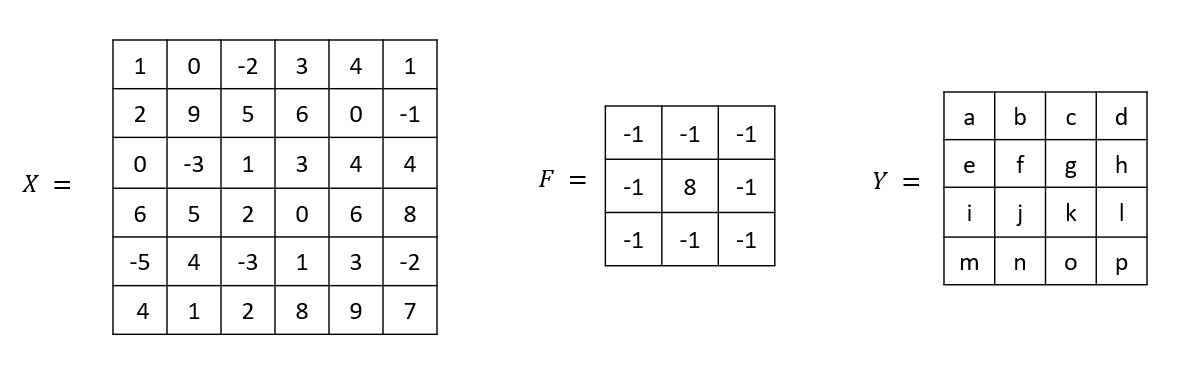
\includegraphics[scale=0.6]{figs/CNN.PNG}
\end{figure}
    \begin{subparts}
    \subpart[1] Let an image $X$ $(6\times6)$ be convolved with a filter $F$ $(3\times3)$ using no padding and a stride of $1$ to produce an output $Y$  $(4\times4$). What is value of $j$ in the output $Y$?\\
    \begin{your_solution}[height=2cm,width=4cm]
    % YOUR ANSWER 
    \end{your_solution}
    
    \vspace{4mm}
    
    \subpart[1] Suppose you instead had an input feature map (or image) of size $6 \times 4$ (height $\times$ width) and a filter of size $2 \times 2$, using no padding and a stride of $2$, what would be the resulting output size? Write your answer in the format: height $\times$ width.\\
    \begin{your_solution}[height=2cm,width=4cm]
    % YOUR ANSWER 
    \end{your_solution} 
    \end{subparts}


% \break

\part Parameter sharing is a very important concept for CNN  because it drastically reduces the complexity of the learning problem and consequently that of the model required to tackle it. The following questions will deal with parameter sharing. Assume that there is no bias term in our convolutional layer.

\begin{subparts}
    \subpart[1] \sall Which of the following are parameters of a convolutional layer?
    \checkboxchar{$\Box$} \checkedchar{$\blacksquare$}
    \begin{checkboxes}
        % YOUR ANSWER 
        % Change \choice to \CorrectChoice for the appropriate selection
        \choice Stride size
        \choice Padding size
        \choice Image size
        \choice Filter size
        \choice Weights in the filter
        \choice None of the above
    \end{checkboxes}
    
    \vspace{4mm}
    
    \subpart[1] \sall Which of the following are hyperparameters of a convolutional layer?
    \checkboxchar{$\Box$} \checkedchar{$\blacksquare$}
    \begin{checkboxes}
        % YOUR ANSWER 
        % Change \choice to \CorrectChoice for the appropriate selection
        \choice Stride size
        \choice Padding size
        \choice Image size
        \choice Filter size
        \choice Weights in the filter
        \choice None of the above
    \end{checkboxes}
    
    \vspace{4mm}

    \subpart[1] Suppose for the convolutional layer, we are given grayscale images of size $22\times 22$. Using one single $4 \times 4$ filter with a stride of $2$ and no padding, what is the \textbf{number of parameters} you are learning in this layer? \\
    \begin{your_solution}[height=2cm,width=4cm]
        % YOUR ANSWER 
    \end{your_solution}\\
    
    \vspace{4mm}
    
    \subpart[1] Now suppose we do not do parameter sharing. That is, each output pixel of this layer is computed by a separate $4 \times 4$ filter. Again we use a stride of $2$ and no padding. What is the \textbf{number of parameters} you are learning in this layer? \\
    \begin{your_solution}[height=2cm,width=4cm]
        % YOUR ANSWER 
    \end{your_solution}

    \newpage
    
    \subpart[1] Now suppose you are given a $40 \times 40$ colored image, which consists of $3$ channels, each representing the intensity of one primary color (so your input is a $40 \times 40 \times 3$ tensor). Once again, you attempt to produce an output map without parameter sharing, using a unique $4 \times 4$ filter per output pixel, with a stride of $2$ and no padding. What is the number of parameters you are learning in this layer? \\
    \begin{your_solution}[height=2cm,width=4cm]
        % YOUR ANSWER 
    \end{your_solution}\\

    \vspace{4mm}

    \subpart[1] In \textit{one concise sentence}, describe a reason why parameter sharing is a good idea for a convolutional layer applied to image data, besides the reduction in number of learned parameters.  \\
    \begin{your_solution}[height=5cm]
        % YOUR ANSWER 
    \end{your_solution}\\
\end{subparts}

\vspace{4mm}

\part Neural the Narwhal was expecting to implement a CNN for Homework 5, but he is disappointed that he only got to write a simple fully-connected neural network. 
\begin{subparts}

\subpart[2] Neural decides to implement a CNN himself and comes up with the following naive implementation:
\begin{lstlisting}[language=Python,escapechar=@]
# image X has shape (H_in, W_in), and filter F has shape (K, K)
# the output Y has shape (H_out, W_out)
Y = np.zeros((H_out, W_out))
for r in range(H_out):
    for c in range(W_out):
        for i in range(K):
            for j in range(K):
                Y[r, c] += X[@\underline{$~~~\emph{\texttt{blank}}~~~$}@] * F[i, j]
\end{lstlisting}
What should be in the \textit{blank} above so that the output \texttt{Y} is correct? Assume that \texttt{H\_out} and \texttt{W\_out} are pre-computed correctly. \\
    \begin{your_solution}[height=1.75cm]
    % YOUR ANSWER 
    % Put your solution in the your_code_solution environment
    \begin{your_code_solution}


    \end{your_code_solution}
    
    \end{your_solution}

\newpage

\subpart[2] Neural now wants to implement the backpropagation part of the network but is stuck. He decides to go to office hours to ask for help. One TA tells him that a CNN can actually be implemented using matrix multiplication. He receives the following 1D convolution example:
\begin{quote}
    Suppose you have an input vector $\xv = [x_1, x_2, x_3, x_4, x_5]^T$ and a 1D convolution filter $\wv = [w_1, w_2, w_3]^T$. Then if the output is $\yv = [y_1, y_2, y_3]^T$, $y_1 = w_1 x_1 + w_2 x_2 + w_3 x_3$, $y_2 = \cdots$, $y_3 = \cdots$. If you look at this closely, this is equivalent to
    \[
    \begin{bmatrix} y_1 \\ y_2 \\ y_3 \end{bmatrix} = \Av \begin{bmatrix} x_1 \\ x_2 \\ x_3 \\ x_4 \\ x_5 \end{bmatrix}
    \]
    where the matrix $\Av$ is given as $\cdots$
\end{quote}
What is matrix $\Av$ for this $\xv$, $\yv$ and $\wv$? Write only the final answer. Your work will \textit{not} be graded. \\
    \begin{your_solution}[height=5cm]
        % YOUR ANSWER 
        % Use `bmatrix` to typeset a matrix.
        % Example:
        % \[
        % \begin{bmatrix}
        % 1 & 2 & 3 \\
        % 4 & 5 & 6
        % \end{bmatrix}
        % \]
        % is a 2 x 3 matrix where the first row has elements 1, 2, 3 and the first column has elements 1, 4.
        % Make sure you put the bmatrix in something like \[ ... \] or in $ ... $
    
    
    \end{your_solution}

\vspace{5mm}

\subpart[2] Neural wonders why the TA told him about matrix multiplication when he wanted to write the backpropagation part. Then he notices that the gradient is extremely simple with this version of CNN. Explain in \textit{one concise sentence (or one short mathematical expression)} how you can compute $\frac{\partial \yv}{\partial \xv}$ once you obtain $\Av$ for some \textit{arbitrary} input $\xv$, filter $\wv$, and the corresponding 1D convolution output $\yv$ (so $\Av$ is obtained following the same procedure as in part (b), but $\xv$, $\yv$ and $\wv$ can be different from the example). Write only the final answer. Your work will \textit{not} be graded. \\
    \begin{your_solution}[height=2cm]
        % YOUR ANSWER 
    
    
    \end{your_solution}


\end{subparts}

\end{parts}

\newpage\newpage

\sectionquestion{Recurrent Neural Network}
\label{sec:rnn}
\begin{parts}

\part Consider the following simple RNN architecture:
\begin{center}

\begin{tikzcd}[cells={nodes={draw=gray}}]
	& {\hat{y}_1} & {\hat{y}_2} & {\hat{y}_3} \\
	{h_0} & {h_1} & {h_2} & {h_3} \\
	& {x_1} & {x_2} & {x_3}
	\arrow[from=2-1, to=2-2]
	\arrow[from=2-2, to=2-3]
	\arrow[from=2-3, to=2-4]
	\arrow[from=3-4, to=2-4]
	\arrow[from=3-3, to=2-3]
	\arrow[from=3-2, to=2-2]
	\arrow[from=2-2, to=1-2]
	\arrow[from=2-3, to=1-3]
	\arrow[from=2-4, to=1-4]
\end{tikzcd}
\end{center}
Where the layers and their corresponding weights are given below:
\begin{align*}
    \xv_t &\in \mathbb{R}^3 &\Wv_{hx} &\in \mathbb{R}^{4 \times 3}\\
    \hv_t &\in \mathbb{R}^4 &\Wv_{hy} &\in \mathbb{R}^{2 \times 4}\\
    \yv_t, \hat{\yv}_t &\in \mathbb{R}^2 &\Wv_{hh} &\in \mathbb{R}^{4 \times 4}\\
\end{align*}\begin{align*}
    J &= \sum_{t=1}^3 J_t\\
    J_t &= -\sum_{i=1}^2 y_{t,i} \log(\hat{y}_{t,i})\\
    \hat{\yv}_t &= \sigma(\ov_t)\\
    \ov_t &= \Wv_{hy}\hv_t\\
    \hv_t &= \psi(\zv_t)\\
    \zv_t &= \Wv_{hh} \hv_{t-1} + \Wv_{hx}\xv_t\\
\end{align*}
Where $\sigma$ is the \textbf{softmax} activation and $\psi$ is the \textbf{identity} activation (i.e. no activation). Note here that we assume that we have no intercept term. $J$ here is computing the cross entropy loss with function $CE()$. $t$ here indicates timesteps.
\begin{subparts}


    \subpart[4] You will now construct the unrolled computational graph for the given model.
    % \emph{(Hint: think about how you can express the recurrence in the model through clever placement of the directed edges in the graph, rather than separating the graph out across timesteps.)}. 
    Use input $\xv$, label $\yv$, and the RNN equations presented above to complete the graph by filling in the solution boxes for the corresponding blanks.\\

    \begin{center}
    \[\begin{tikzcd}[cells={nodes={draw=gray}}]
	&& {J = \sum_{t=1}^3 J_t} \\
	&& {W_{hy}} \\
	&& {y_2} & {y_3} \\
	{y_1} & {J_1 = CE(\hat{y}_{1}, y_1)} & {\textbf{part c}} & {J_3 = CE(\hat{y}_{3}, y_3)} \\
	& {\hat{y}_1 = \sigma(o_1)} & {\hat{y}_2 = \sigma(o_2)} & {\hat{y}_3 = \sigma(o_3)} \\
	& {\textbf{part a}} & {o_2 = Lin(W_{hy}, h_2)} & {o_3 = Lin(W_{hy}, h_3)} \\
	& {h_1 = \psi(z_1)} & {\textbf{part b}} & {h_3 = \psi(z_3)} \\
	{h_0} & {z_1 = Lin(W_{hh}, W_{hx},h_0,x_1)} & {z_2 = Lin(W_{hh}, W_{hx},h_1,x_2)} & {\textbf{part d}} \\
	& {x_1} & {x_2} & {x_3} \\
	& {W_{hx}} & {W_{hh}}
	\arrow[from=8-1, to=8-2]
	\arrow[from=9-2, to=8-2]
	\arrow[from=8-2, to=7-2]
	\arrow[from=7-2, to=8-3]
	\arrow[from=7-2, to=6-2]
	\arrow[from=6-2, to=5-2]
	\arrow[from=5-2, to=4-2]
	\arrow[from=4-1, to=4-2]
	\arrow[from=9-3, to=8-3]
	\arrow[from=8-3, to=7-3]
	\arrow[from=7-3, to=6-3]
	\arrow[from=6-3, to=5-3]
	\arrow[from=5-3, to=4-3]
	\arrow[from=3-3, to=4-3]
	\arrow[from=3-4, to=4-4]
	\arrow[from=5-4, to=4-4]
	\arrow[from=6-4, to=5-4]
	\arrow[from=7-4, to=6-4]
	\arrow[from=8-4, to=7-4]
	\arrow[from=7-3, to=8-4]
	\arrow[from=9-4, to=8-4]
	\arrow[shift left=4, from=10-2, to=8-2]
	\arrow[from=10-2, to=8-3]
	\arrow[from=10-3, to=8-2]
	\arrow[shift right=4, from=10-3, to=8-3]
	\arrow[from=10-3, to=8-4]
	\arrow[shift right=2, from=2-3, to=6-4]
	\arrow[from=2-3, to=6-2]
	\arrow[shift right=5, from=2-3, to=6-3]
	\arrow[from=4-2, to=1-3]
	\arrow[shift right=4, from=4-3, to=1-3]
	\arrow[shift right, from=4-4, to=1-3]
	\arrow[shift right=3, from=10-2, to=8-4]
\end{tikzcd}\]
\end{center}
    \begin{your_solution}[title=(a),height=2cm,width=6cm]
    % YOUR ANSWER
    \end{your_solution}
     \begin{your_solution}[title=(b),height=2cm,width=6cm]
    % YOUR ANSWER
    \end{your_solution}\\
     \begin{your_solution}[title=(c),height=2cm,width=6cm]
    % YOUR ANSWER
    \end{your_solution}
     \begin{your_solution}[title=(d),height=2cm,width=6cm]
    % YOUR ANSWER
    \end{your_solution}

\subpart Now you will derive the steps of the backpropagation algorithm that lead to the computation of $\frac{dJ}{dW_{hh}}$. For all parts of this question, please write your answer in terms of $W_{hh}$, $W_{hy}$, $y$, $\hat{y}$, $h$, and any additional terms specified in the question (note: this does not mean that every term listed shows up in every answer, but rather that you should simplify terms into these as much as possible when you can).
    \begin{subsubparts}
        \subsubpart[2] What is $g_{J_t} = \frac{\partial J}{\partial J_t}$? Write your solution in the first box, and show your work in the second.
        
    \begin{your_solution}[title=$\frac{\partial J}{\partial J_t}$,height=2.5cm,width=8.5cm]
    % YOUR ANSWER
    \end{your_solution}
    
    \begin{your_solution}[title=Work,height=6cm,width=14cm]
    % YOUR ANSWER
    \end{your_solution}

     \subsubpart[2] What is $g_{o_t} = \frac{\partial J}{\partial o_t}$? Write your solution in the first box, and show your work in the second. Write your answer in terms of $\hat{y}_t$, $y_t$, and $g_{J_t}$(Hint: Think about how you can write $J_t$ in terms of $o_t$, then use the chain rule. You may want to use a result from homework 5 to help here.)
    
    %\emph{(Hint: First derive the partial derivatives with respective to everything after $h_t$, which should be similar to HW5. After that, try to break up the objective into a term for each timestep.)}
    
    \begin{your_solution}[title=$\frac{\partial J}{\partial \ov_t}$,height=2.5cm,width=8.5cm]
    % YOUR ANSWER
    \end{your_solution}
    
    \begin{your_solution}[title=Work,height=6cm,width=14cm]
    % YOUR ANSWER
    \end{your_solution}
    
    \subsubpart[2] What is $g_{\hv_i} = \frac{\partial J}{\partial \hv_i}$ for an arbitrary $i \in [1,3]$? Write your solution in terms of $\gv_{\ov_t}$, $W_{hh}$, $W_{hy}$ in the first box, and show your work in the second. (Hint: Find $\frac{\partial o_t}{\partial h_i}$, then use the chain rule. Also, for a given i, think about which $o_t$'s  $h_i$ affects)
    
    %\emph{(Hint: First derive the partial derivatives with respective to everything after $h_t$, which should be similar to HW5. After that, try to break up the objective into a term for each timestep.)}
    
    \begin{your_solution}[title=$\frac{\partial J}{\partial \hv_i}$,height=2.5cm,width=8.5cm]
    % YOUR ANSWER
    \end{your_solution}
    
    \begin{your_solution}[title=Work,height=6cm,width=14cm]
    % YOUR ANSWER
    \end{your_solution}
    
    \subsubpart[2] What is $g_{\Wv_{hh}} = \frac{\partial J}{\partial \Wv_{hh}}$? Write your solution in terms of $\gv_{\hv_i}$ and $h$ in the first box, and show your work in the second (Hint: $W_{hh}$ is in every timestep, so you need to consider that in the derivative).
    
    
    \begin{your_solution}[title=$\frac{\partial J}{\partial W_{hh}}$,height=2.5cm,width=10.5cm]
    % YOUR ANSWER
    \end{your_solution}
    
    \begin{your_solution}[title=Work,height=8.5cm,width=14cm]
    % YOUR ANSWER
    \end{your_solution}
    
    \end{subsubparts}
    
\end{subparts}


\newpage
\part[2] \sall Which of the following are true about RNN and RNN-LM?
    
    {%
    \checkboxchar{$\Box$} \checkedchar{$\blacksquare$}
    \begin{checkboxes}
        
        \choice An RNN cannot process sequential data, whereas an RNN-LM is designed for sequential data processing such as in natural language processing.

        \choice An RNN-LM is only exclusively used as an encoder, which can process sequential data and encode it into a fixed-size state vector.

        \choice An RNN-LM includes additional layers and structures specifically designed to predict the next token in a sequence, making it more suited for tasks like text generation than a standard RNN.

        \choice The RNN-LM is trained to maximize the probability of a sequence of tokens, given a previous sequence, which is not a typical training objective of a standard RNN.
        
        \choice None of the above.
    \end{checkboxes}
    }
    

\end{parts}

\newpage

\newpage
\sectionquestion{Transformers and AutoDiff}
\label{sec:transformers}

\begin{parts}

\part[1] 
\begin{figure}[h]
    \centering
    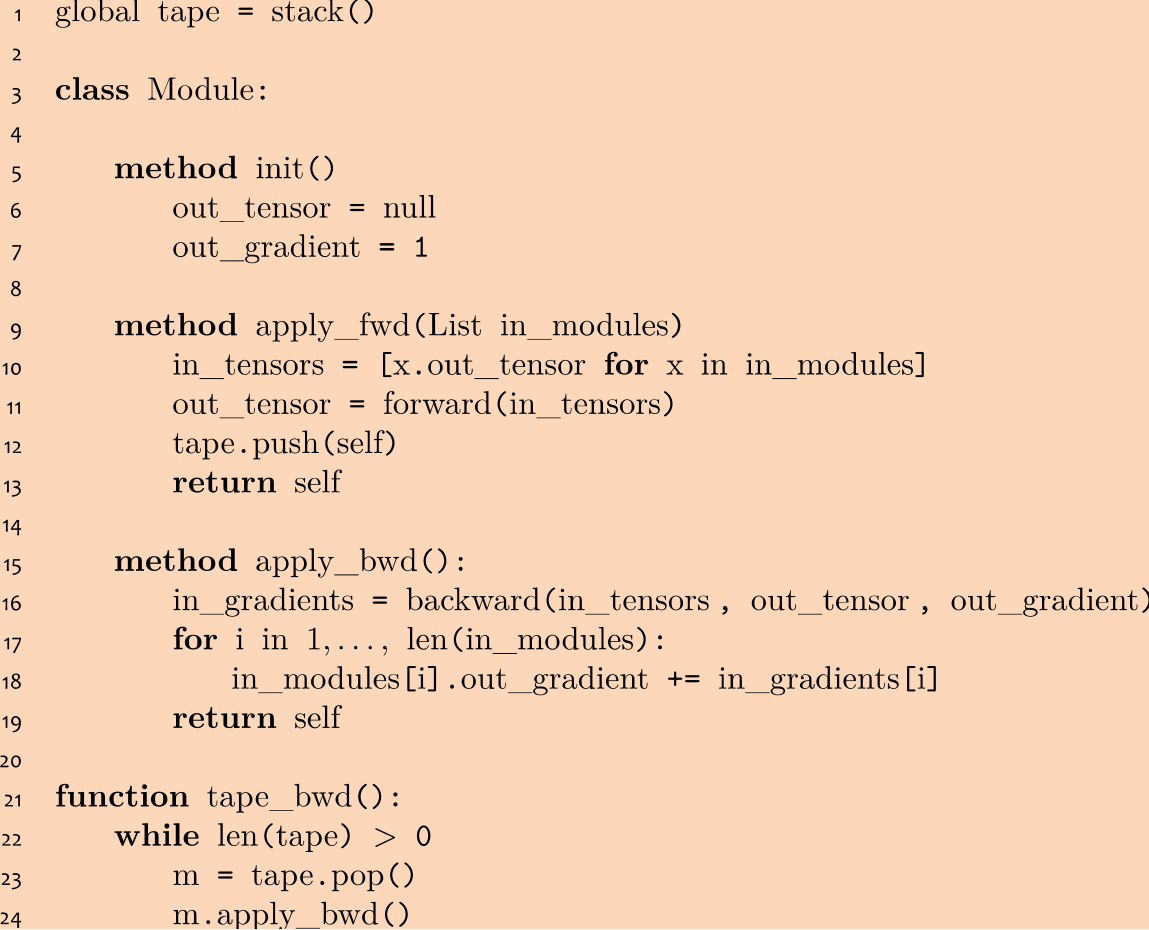
\includegraphics[scale=0.6]{figs/autodiff.png}
\end{figure}

\textbf{Select one:} This is a code snippet from lecture 18 slide 16. In the context of the \texttt{method apply\_fwd()} inside the \texttt{Module} class, what is the primary role of the \texttt{tape.push(self)} command that pushes the module onto the tape?

    \begin{list}{}
    % YOUR ANSWER
    % Change \emptycircle to \filledcircle for the appropriate selection/selections
        \item 
            \emptycircle
            % \filledcircle
            It records the current module onto the stack along with its parameters and tensors to ensure that the output tensor is saved for the backward pass.
        \item 
            \emptycircle 
            % \filledcircle
            It pushes the current computation's gradient onto the stack for immediate use in the forward pass.

        \item 
            \emptycircle
            % \filledcircle
            It duplicates the module to allow for parallel computations in subsequent layers of the neural network.
 
        \item 
            \emptycircle
            % \filledcircle
            It activates the module for the forward pass, making it the only active computation in the network.
    \end{list}
    

\part[2]  
\textbf{True or False:} We can replace a stack with a queue in Module-based AutoDiff. Explain your reasoning in no more than 2 sentences in the box below.
    \begin{list}{}
    % YOUR ANSWER
    % Change \emptycircle to \filledcircle for the appropriate selection/selections
        \item 
            \emptycircle
            % \filledcircle
            True 
        \item 
            \emptycircle 
            % \filledcircle
            False 
    \end{list}

\begin{your_solution}[height=3cm, width=\textwidth]
\end{your_solution}

\part[2]  
We are looking to replace Neural the Narwhal with another mascot that is \textbf{cute and efficient}. We would want you to use a transformer that helps us decide a \textbf{mascot name} by searching in a large pool of possible mascots. How would the transformer help decide which mascot to choose? Suggest a possible \textbf{key}, \textbf{value} pair that it would consider.  Be specific about which is the key and which is the value. \\ 
Hint: When you conduct a search on a web search engine (e.g. Google), the search engine compares your entered query with a set of \textbf{keys} (e.g. webpage titles, content, and metadata) of web pages in its database. It then displays the most relevant web pages as search results (\textbf{values}).


\begin{your_solution}[height=5cm, width=\textwidth]
\end{your_solution}
\vspace{1cm}

% (Just kidding. We would never replace Neural the Narwhal!)

\part 
Consider a Transformer model employing a multi-headed self-attention mechanism. Suppose the input consists of a sequence of $T$ tokens, each token represented by a $d_{\text{model}}$-dimensional embedding vector. This model utilizes $H$ attention heads. During the attention process, each head generates key, query, and value matrices from the input embeddings. The dimensionality of the key and query vectors is $d_k$ for each head, and the attention function produces an output vector of dimension $d_v$ for each token and head.

\begin{subparts}

\subpart[1] Which of the following represents the dimension of the key matrix for a single attention head?

    \begin{list}{}
    % YOUR ANSWER
    % Change \emptycircle to \filledcircle for the appropriate selection/selections
        \item 
            \emptycircle
            % \filledcircle
            $T \times d_v$
        \item 
            \emptycircle 
            % \filledcircle
            $H \times d_k \times d_{\text{model}}$
        \item 
            \emptycircle 
            % \filledcircle
            $T \times d_k$
        \item 
            \emptycircle 
            % \filledcircle
            $T \times d_{\text{model}} \times d_k$
    \end{list}


\subpart[1]  Which of the following represents the dimension of the output matrix of the multi-headed attention before any final linear transformation?

    \begin{list}{}
    % YOUR ANSWER
    % Change \emptycircle to \filledcircle for the appropriate selection/selections
        \item 
            \emptycircle
            % \filledcircle
            $T \times H \times d_k$
        \item 
            \emptycircle 
            % \filledcircle
            $T \times H \times d_v$
        \item 
            \emptycircle 
            % \filledcircle
            $T \times d_{\text{model}}$
        \item 
            \emptycircle 
            % \filledcircle
            $H \times d_k \times d_v$
    \end{list}


\end{subparts}
\end{parts}
\newpage
\sectionquestion{Pre-training, Fine-tuning, In-context Learning}
\label{sec:pretrain_finetune}

\begin{parts}

\part[2] Select the correct statements about the pre-training and fine-tuning phases:

    {%
    \checkboxchar{$\Box$} \checkedchar{$\blacksquare$}
    \begin{checkboxes}
        \choice The pre-training dataset usually requires a large amount of labeled data to guide the initial learning process and shape the weight configurations.

        \choice The fine-tuning dataset is typically much larger than the pre-training dataset and contains a wide variety of examples from numerous domains to ensure that the model can generalize well to any task.

        \choice Reconstruction error is a metric used during the fine-tuning process to measure the accuracy of a model's predictions, typically calculated as the percentage of correct labels the model assigns during supervised learning tasks
        
        \choice None of the above.
    \end{checkboxes}
    }
    

\part[2] Select the correct statements about in-context learning:

    {%
    \checkboxchar{$\Box$} \checkedchar{$\blacksquare$}
    \begin{checkboxes}
        \choice Zero-shot learning models usually make accurate predictions for tasks they have not explicitly been trained for, relying solely on a rich, pre-trained representation of data.

        \choice One-shot learning models require only a single example to learn a new task, often leveraging this example to make analogies and predictions for similar tasks.

        \choice Few-shot learning models typically require thousands of examples to learn a new task effectively and are not practical for data-scarce scenarios.

        \choice In-context learning requires updating the model's parameters with gradient descent on each new example to make accurate predictions.
        
        \choice None of the above.
    \end{checkboxes}
    }
    
    

\part[3] Llama2 (\href{https://www.llama2.ai/}{https://www.llama2.ai/}) is Meta's open source large language model. Interact with llama2 with your own topic of choice (Please try to stick to simple mathematical operations to do your analysis). In the answer box below, put the prompt and the output from Llama2 for (1) a zero-shot scenario and (2) a few-shot in-context learning scenario in which the zero-shot provides poor feedback but the few-shot performs better. Summarize what you observe in one sentence.

\begin{your_solution}[height=20cm, width=\textwidth]
\end{your_solution}

\end{parts}
\newpage
\sectionquestion{Empirical Questions}
\label{sec:empirical}

The following questions should be completed as you work through the programming component of this assignment. \textbf{Please ensure that all plots are computer-generated}. 

\begin{parts}
\part[3]  Plot the \textbf{training loss} against \textbf{number of iterations} during pre-training. The code provided automatically prints the loss every 2000 iterations.

\begin{your_solution}[height=9cm]
% YOUR ANSWER 
\begin{center}
% Here is an example of how to include an image:
% \includegraphics{IMAGE FILE PATH HERE}
\end{center}
\end{your_solution}

\newpage
\part[5] Plot the \textbf{validation accuracy} for training sizes [16, 32, 64, 128, 256, 512] for your fine-tuned model with pre-training and without pre-training. Please put them in the same plot.\\


\begin{your_solution}[height=9cm]
% YOUR ANSWER 
\begin{center}
% Here is an example of how to include an image:
% \includegraphics{IMAGE FILE PATH HERE}
\end{center}
\end{your_solution}



\end{parts}\newpage
\end{questions}
\newpage
\section{Collaboration Questions}
After you have completed all other components of this assignment, report your answers to these questions regarding the collaboration policy. Details of the policy can be found \href{http://www.cs.cmu.edu/~mgormley/courses/10601/syllabus.html}{here}.
\begin{enumerate}
    \item Did you receive any help whatsoever from anyone in solving this assignment? If so, include full details.
    \item Did you give any help whatsoever to anyone in solving this assignment? If so, include full details.
    \item Did you find or come across code that implements any part of this assignment? If so, include full details.
\end{enumerate}

\begin{your_solution}[height=6cm]
% YOUR ANSWER 

\end{your_solution}

\newpage

\section{Programming (30 points)}
\label{programming}

\subsection{The Task}\label{task}
In the programming section you will partially implement a transformer, pre-train it on WikiText2 dataset and fine-tune it for sentiment analysis on movie reviews.
On a technical level the main task is to implement the attention layer of the transformer, pre-train and fine-tune the model, and evaluate if pre-training helps improve performance or not. 

The link to the python notebook \texttt{transformer.ipynb} is \href{https://colab.research.google.com/drive/1tAUgpgrJyO4orWbCdX5AU07c8cVMe8dU?usp=sharing}{here}. Use your CMU Google Account to access the file. Make a copy of the file by clicking on the File button on the top left corner (right below the file name) and select "Save a Copy in Drive". Work on that copy and upload your completed transformer.ipynb file to Gradescope.

\subsection{The Dataset}\label{dataset}
\href{https://paperswithcode.com/dataset/wikitext-2}{WikiText2} dataset is a publicly available dataset used for pretraining in this notebook, which is a collection of over 2 million words extracted from Wikipedia articles and is commonly used for language modeling tasks.

\subsubsection{Data Preparation}\label{dataset}
The dataset is prepared using SentencePiece, a text tokenizer and detokenizer mainly used for Neural Network Machine Translation applications. In this notebook, SentencePiece is utilized to generate a tokenizer model from the Wikitext training tokens, and this model is used for tokenizing the dataset into subword units (Byte Pair Encoding - BPE). The vocabulary size is set to 50,000, which is a common size for many language tasks.

\subsubsection{Data Loading and Batching}\label{dataset}
A custom Corpus class is defined to handle the loading and numericalization of the tokens from the dataset files. The class reads and processes the following files:

\texttt{wiki.train.tokens}\\
\texttt{wiki.valid.tokens}\\
\texttt{wiki.test.tokens}\\
These files contain the training, validation, and test sets respectively, with tokens already preprocessed and separated by spaces.

For training purposes, the notebook defines functions to generate random and sequential batches of these tokens. The batch size and sequence length are configurable, but as an example, the notebook uses a batch size of 32 and a sequence length of 65 tokens.

\subsubsection{Data Iteration}\label{dataset}
Two types of batch samplers are used:

\textbf{random\_batch\_sampler:} Generates random batches of tokens, which is often used in training to introduce stochasticity.\\
\textbf{sequential\_batch\_sampler:} Generates batches of tokens sequentially, which can be useful for validation and testing to preserve the sequence order.\\
\newline
Both samplers ensure that the tokens are appropriately batched and placed onto the correct device (CPU or GPU) for model training.

\subsubsection{File Format}\label{dataset}
The text data in the dataset files is raw and unstructured, requiring the Corpus class to handle tokenization and numericalization. We use subword tokenization to ensure there are not out-of-vocabulary words.

\subsection{Learning}
Your first task is to implement the multi-headed attention layer to complete the implementation of the transformer model. This implementation should be designed to integrate with the existing model architecture provided in the notebook. The attention layer is critical for the model to weigh the importance of different tokens in the input sequence when predicting the next token.

This layer will compute dynamic weights for different parts of the input sequence, thereby allowing the model to prioritize which information to attend to during the learning process.

\[
\text{Attention}(Q, K, V) = \text{softmax}\left(\frac{QK^T}{\sqrt{d_k}}\right)V
\]
Where\\
\setlength{\parindent}{20pt} %
\indent \text{\( Q \) represents the matrix of queries.}\\
\indent \text{\( K \) represents the matrix of keys.}\\
\indent \text{ \( V \) represents the matrix of values.}\\
\indent \text{\( d_k \) is the dimensionality of the keys and queries.}\\
\newline
Note: There are hints and TODOs to guide you through the implementation. While implementing if you plan to use any helper function, define it in the same cell where it is being called.  The reference implementation takes around 1 hour to complete pre-training.

\subsection{Transformer Architecture for Pre-training and Fine Tuning}
\subsubsection{Transformer Language Model (TransformerLM)}
The Transformer class defines a standard transformer architecture primarily used for language modeling tasks. This model takes a sequence of token indices (representing words or subwords in a sentence) as input and predicts the next token in the sequence. Key components include:\\
\newline
\textbf{Embedding Layer:} Converts token indices (which are numerical representations of words) into dense vector representations. These dense vectors capture more nuanced information about words than mere indices, allowing the model to understand word meanings and relationships.\\
\newline
\textbf{Positional Encoding:} Adds information about the position of each token in the sequence.  This helps the model understand the order of words in a sentence, which is crucial for interpreting the meaning correctly. It's essential because the model processes input in parallel and doesn't inherently capture sequential information. \\
\newline
\textbf{Decoder Layers:} \\
\textbf{Multi-Head Attention} layer allows the model to focus on different parts of the input sentence simultaneously, capturing different types of relationships between words. It's implemented through the MultiHeadAttention class, which splits the input into multiple heads, allowing the model to attend to different segments of the input simultaneously.\\ \textbf{Position-Wise FeedForward} layer applies a simple neural network to each position's output from the attention mechanism, further processing the information.\\
\newline
\textbf{Output Layer:} Transforms the final output of the decoder layers into a format that matches the size of the model's vocabulary.This layer is used for predicting the next word in the sequence, with each element in the output corresponding to a probability score for each word in the vocabulary.\\
\newline
\textbf{Masking:} The generate\_mask function in the Transformer class creates a mask to hide future tokens. This is crucial during training to ensure that the prediction for a particular token doesn’t depend on the future tokens
\subsubsection{Classification Transformer (Fine-Tuning)}
\textbf{Architecture:} The ClassificationTransformer class adapts the pre-trained TransformerLM for a classification task. It reuses the embedding and positional encoding layers from the pre-trained model and adds a final fully connected layer for classification.\\
\newline
\textbf{Adaptations for Classification:}\\
\textbf{Reuses Pre-Trained Components:} Embeddings and positional encodings from the pre-trained model are directly utilized, leveraging the knowledge acquired during the language modeling phase.\\
\textbf{Final Classification Layer:} A linear layer that takes the output of the last token (or a special classification token) and projects it to the number of classes for classification tasks.\\

\subsection{Training and Evaluation:}
\subsubsection{Pre-Training}
\textbf{Forward Pass:}The model processes the input data and generates predictions for the next token.\\
\textbf{Loss Calculation:} The Cross-Entropy Loss between the predictions and the actual next tokens is computed.\\
\textbf{Backpropagation:} The gradients of the loss are calculated and used to update the model’s weights.\\
\textbf{Optimizer:} An optimizer like Adam is commonly used to adjust the weights to minimize the loss.\\
\subsubsection{Fine-Tuning Process}
\textbf{Forward Pass:} The input data goes through the model, which now predicts class labels instead of the next word.\\
\textbf{Loss Calculation:} Cross-Entropy Loss is calculated between the predicted labels and the true labels.\\
\textbf{Backpropagation and Optimization:} Similar to the pre-training phase, but the focus is more on fine-tuning the weights, especially in the newly added output layer.\\
\newline
\textbf{ Please make sure that you use \texttt{to(device)}}\\
Need for \texttt{to(device)}: These calls ensure that the model and data are moved to the GPU, which provides faster computation compared to a CPU, especially beneficial for training large models like Transformers. Pre-training a Transformer model is a computationally intensive task due to the model's size and complexity, and the large size of the training datasets. Utilizing a GPU significantly speeds up this process.
\subsection{Gradescope Submission}
You should submit your \texttt{transformer.ipynb} to Gradescope. \textbf{Any other files will be deleted.} Please do not use other file names. Do not modify cells that does not explicitly say so.  
Some additional tips: 
For this programming assignment most of the implementation is provided to you and following the hints and TODOs carefully should help you get through them.




\end{document}
